\documentclass{standalone}
\usepackage{tikz}
\usetikzlibrary{patterns, positioning}


\begin{document}
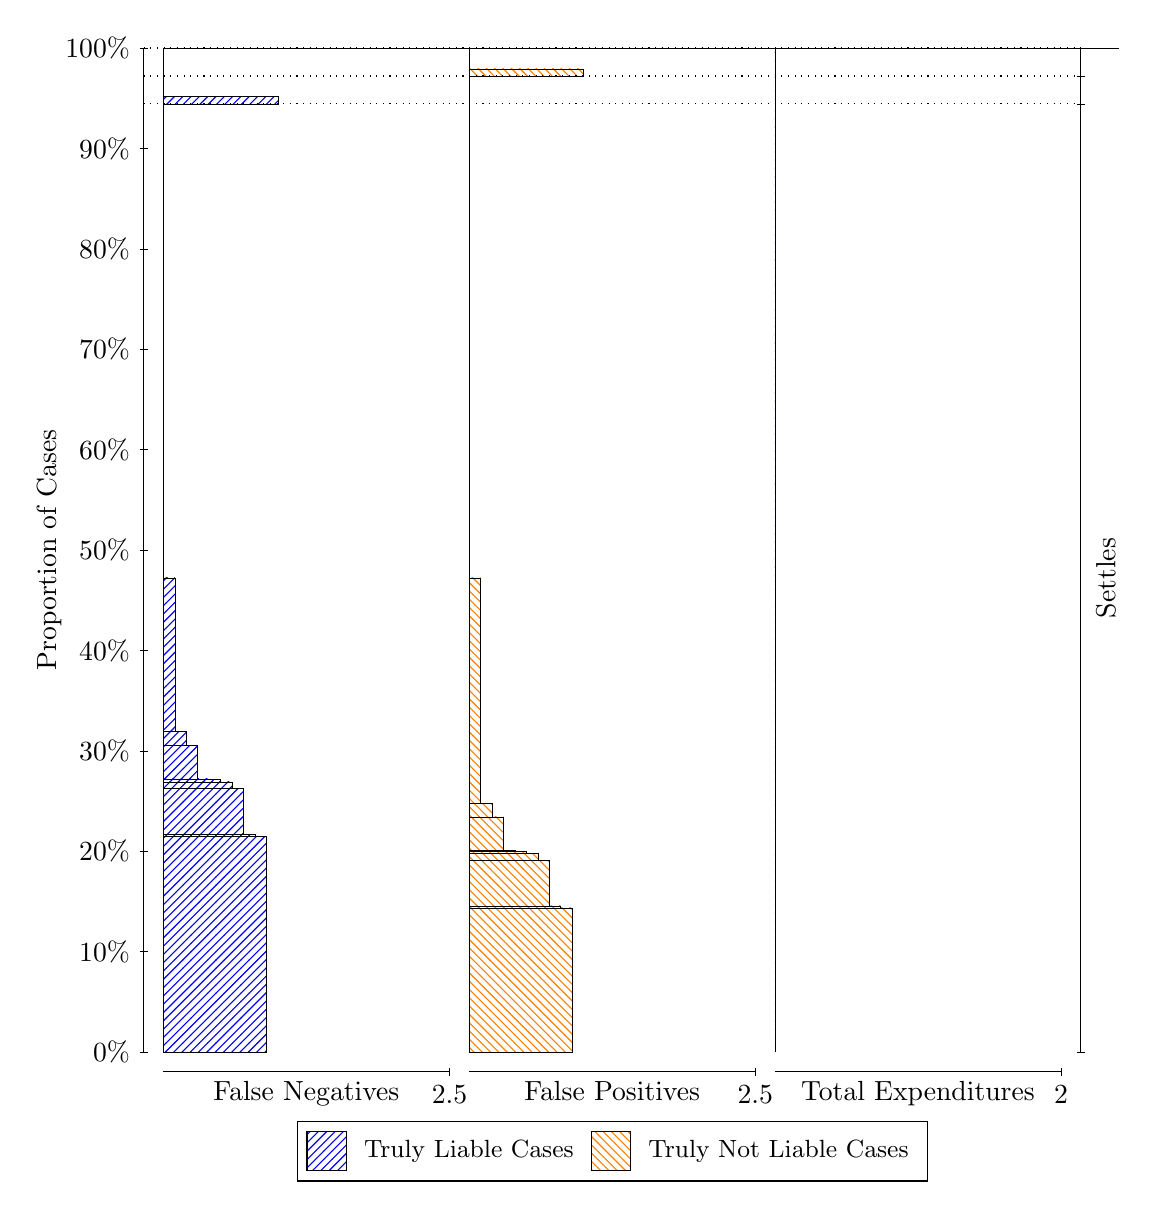
\begin{tikzpicture}
\draw[black, very thin] (1.5,1.75) -- (1.5,14.5);
\node[rotate=90, text=black, anchor=center] at (0.3, 8.125) {Proportion of Cases};
\draw[black, very thin] (1.45,1.75) -- (1.55,1.75);
\node[text=black, anchor=east] at (1.45, 1.75) {0\%};
\draw[black, very thin] (1.45,3.025) -- (1.55,3.025);
\node[text=black, anchor=east] at (1.45, 3.025) {10\%};
\draw[black, very thin] (1.45,4.3) -- (1.55,4.3);
\node[text=black, anchor=east] at (1.45, 4.3) {20\%};
\draw[black, very thin] (1.45,5.575) -- (1.55,5.575);
\node[text=black, anchor=east] at (1.45, 5.575) {30\%};
\draw[black, very thin] (1.45,6.85) -- (1.55,6.85);
\node[text=black, anchor=east] at (1.45, 6.85) {40\%};
\draw[black, very thin] (1.45,8.125) -- (1.55,8.125);
\node[text=black, anchor=east] at (1.45, 8.125) {50\%};
\draw[black, very thin] (1.45,9.4) -- (1.55,9.4);
\node[text=black, anchor=east] at (1.45, 9.4) {60\%};
\draw[black, very thin] (1.45,10.675) -- (1.55,10.675);
\node[text=black, anchor=east] at (1.45, 10.675) {70\%};
\draw[black, very thin] (1.45,11.95) -- (1.55,11.95);
\node[text=black, anchor=east] at (1.45, 11.95) {80\%};
\draw[black, very thin] (1.45,13.225) -- (1.55,13.225);
\node[text=black, anchor=east] at (1.45, 13.225) {90\%};
\draw[black, very thin] (1.45,14.5) -- (1.55,14.5);
\node[text=black, anchor=east] at (1.45, 14.5) {100\%};

\draw[black, very thin] (13.4,1.75) -- (13.4,14.5);
\draw[black, very thin] (13.35,1.75) -- (13.45,1.75);
\node[anchor=west] at (13.35, 1.75) {};
\draw[black, very thin] (13.35,13.79) -- (13.45,13.79);
\node[anchor=west] at (13.35, 13.79) {};
\draw[black, very thin] (13.35,14.145) -- (13.45,14.145);
\node[anchor=west] at (13.35, 14.145) {};
\draw[black, very thin] (13.35,14.499) -- (13.45,14.499);
\node[anchor=west] at (13.35, 14.499) {};
\draw[black, very thin] (13.35,14.5) -- (13.45,14.5);
\node[anchor=west] at (13.35, 14.5) {};
\draw[black, very thin] (13.35,14.5) -- (13.45,14.5);
\node[anchor=west] at (13.35, 14.5) {};

\draw[black, very thin, pattern color=blue, pattern=north east lines] (1.75,1.75) rectangle (3.058,4.4908);
\draw[black, very thin, pattern color=blue, pattern=north east lines] (1.75,4.4908) rectangle (2.9127,4.5173);
\draw[black, very thin, pattern color=blue, pattern=north east lines] (1.75,4.5173) rectangle (2.7673,5.0931);
\draw[black, very thin, pattern color=blue, pattern=north east lines] (1.75,5.0931) rectangle (2.622,5.1799);
\draw[black, very thin, pattern color=blue, pattern=north east lines] (1.75,5.1799) rectangle (2.4767,5.2071);
\draw[black, very thin, pattern color=blue, pattern=north east lines] (1.75,5.2071) rectangle (2.3313,5.2186);
\draw[black, very thin, pattern color=blue, pattern=north east lines] (1.75,5.2186) rectangle (2.186,5.646);
\draw[black, very thin, pattern color=blue, pattern=north east lines] (1.75,5.646) rectangle (2.0407,5.8204);
\draw[black, very thin, pattern color=blue, pattern=north east lines] (1.75,5.8204) rectangle (1.8953,7.7701);
\draw[black, very thin, pattern color=orange, pattern=north west lines] (1.75,7.7701) rectangle (1.75,13.79);
\draw[black, very thin, pattern color=blue, pattern=north east lines] (1.75,13.79) rectangle (3.2033,13.881);
\draw[black, very thin, pattern color=orange, pattern=north west lines] (1.75,13.881) rectangle (1.75,14.145);
\draw[black, very thin, pattern color=orange, pattern=north west lines] (1.75,14.145) rectangle (1.75,14.236);
\draw[black, very thin, pattern color=blue, pattern=north east lines] (1.75,14.236) rectangle (1.75,14.499);
\draw[black, very thin, pattern color=blue, pattern=north east lines] (1.75,14.499) rectangle (6.6913,14.499);
\draw[black, very thin, pattern color=orange, pattern=north west lines] (1.75,14.499) rectangle (1.75,14.5);
\draw[black, very thin, pattern color=orange, pattern=north west lines] (1.75,14.5) rectangle (1.75,14.5);
\draw[black, very thin, pattern color=blue, pattern=north east lines] (1.75,14.5) rectangle (1.75,14.5);
\draw[black, very thin, pattern color=orange, pattern=north west lines] (5.6333,1.75) rectangle (6.9413,3.5802);
\draw[black, very thin, pattern color=orange, pattern=north west lines] (5.6333,3.5802) rectangle (6.796,3.6066);
\draw[black, very thin, pattern color=orange, pattern=north west lines] (5.6333,3.6066) rectangle (6.6507,4.1825);
\draw[black, very thin, pattern color=orange, pattern=north west lines] (5.6333,4.1825) rectangle (6.5053,4.2692);
\draw[black, very thin, pattern color=orange, pattern=north west lines] (5.6333,4.2692) rectangle (6.36,4.2964);
\draw[black, very thin, pattern color=orange, pattern=north west lines] (5.6333,4.2964) rectangle (6.2147,4.308);
\draw[black, very thin, pattern color=orange, pattern=north west lines] (5.6333,4.308) rectangle (6.0693,4.7353);
\draw[black, very thin, pattern color=orange, pattern=north west lines] (5.6333,4.7353) rectangle (5.924,4.9097);
\draw[black, very thin, pattern color=orange, pattern=north west lines] (5.6333,4.9097) rectangle (5.7787,7.7703);
\draw[black, very thin, pattern color=blue, pattern=north east lines] (5.6333,7.7703) rectangle (5.6333,13.79);
\draw[black, very thin, pattern color=orange, pattern=north west lines] (5.6333,13.79) rectangle (5.6333,14.054);
\draw[black, very thin, pattern color=blue, pattern=north east lines] (5.6333,14.054) rectangle (5.6333,14.145);
\draw[black, very thin, pattern color=orange, pattern=north west lines] (5.6333,14.145) rectangle (7.0867,14.236);
\draw[black, very thin, pattern color=blue, pattern=north east lines] (5.6333,14.236) rectangle (5.6333,14.499);
\draw[black, very thin, pattern color=orange, pattern=north west lines] (5.6333,14.499) rectangle (5.6333,14.499);
\draw[black, very thin, pattern color=blue, pattern=north east lines] (5.6333,14.499) rectangle (5.6333,14.5);
\draw[black, very thin, pattern color=orange, pattern=north west lines] (5.6333,14.5) rectangle (10.575,14.5);
\draw[black, very thin, pattern color=blue, pattern=north east lines] (5.6333,14.5) rectangle (9.1213,14.5);
\draw[black, very thin, pattern color=orange, pattern=north west lines] (9.5167,1.75) rectangle (9.5167,7.7703);
\draw[black, very thin, pattern color=blue, pattern=north east lines] (9.5167,7.7703) rectangle (9.5167,13.79);
\draw[black, very thin, pattern color=orange, pattern=north west lines] (9.5167,13.79) rectangle (9.5167,14.054);
\draw[black, very thin, pattern color=blue, pattern=north east lines] (9.5167,14.054) rectangle (9.5167,14.145);
\draw[black, very thin, pattern color=orange, pattern=north west lines] (9.5167,14.145) rectangle (9.5167,14.236);
\draw[black, very thin, pattern color=blue, pattern=north east lines] (9.5167,14.236) rectangle (9.5167,14.499);
\draw[black, very thin, pattern color=orange, pattern=north west lines] (9.5167,14.499) rectangle (13.877,14.499);
\draw[black, very thin, pattern color=blue, pattern=north east lines] (9.5167,14.499) rectangle (13.877,14.5);
\draw[black, very thin, pattern color=orange, pattern=north west lines] (9.5167,14.5) rectangle (13.877,14.5);
\draw[black, very thin, pattern color=blue, pattern=north east lines] (9.5167,14.5) rectangle (13.877,14.5);
\draw[black, dotted] (1.5,13.79) -- (13.4,13.79);
\draw[black, dotted] (1.5,14.145) -- (13.4,14.145);
\draw[black, dotted] (1.5,14.499) -- (13.4,14.499);
\draw[black, dotted] (1.5,14.5) -- (13.4,14.5);
\draw[black, very thin] (1.75,1.5) -- (5.3833,1.5);
\node[text=black, anchor=north] at (3.5667, 1.5) {False Negatives};
\draw[black, very thin] (5.3833,1.45) -- (5.3833,1.55);
\node[text=black, anchor=north] at (5.3833, 1.45) {2.5};

\draw[black, very thin] (5.6333,1.5) -- (9.2667,1.5);
\node[text=black, anchor=north] at (7.45, 1.5) {False Positives};
\draw[black, very thin] (9.2667,1.45) -- (9.2667,1.55);
\node[text=black, anchor=north] at (9.2667, 1.45) {2.5};

\draw[black, very thin] (9.5167,1.5) -- (13.15,1.5);
\node[text=black, anchor=north] at (11.333, 1.5) {Total Expenditures};
\draw[black, very thin] (13.15,1.45) -- (13.15,1.55);
\node[text=black, anchor=north] at (13.15, 1.45) {2};

\node[text=black, centered, rotate=90] at (13.72, 7.7702) {Settles};





\draw (7.449999999999999,1.5) node[draw=none] (baseCoordinate) {};
\begin{scope}[align=center]
        \matrix[scale=0.5, draw=black, below=0.5cm of baseCoordinate, nodes={draw}, column sep=0.1cm]{
            \node[rectangle, draw, minimum width=0.5cm, minimum height=0.5cm, pattern color=blue, pattern=north east lines] {}; &
            \node[draw=none, font=\small, text=black] (B) {Truly Liable Cases}; &
            \node[rectangle, draw, minimum width=0.5cm, minimum height=0.5cm, pattern color=orange, pattern=north west lines] {}; &
            \node[draw=none, font=\small, text=black] (B) {Truly Not Liable Cases}; \\
            };
\end{scope}

\end{tikzpicture}
\end{document}